\documentclass[a5paper, 10pt]{article}

% Текст
\usepackage[utf8]{inputenc} % UTF-8 кодировка
\usepackage[russian]{babel} % Русский язык
\usepackage{indentfirst} % красная строка в первом параграфе в главе
% Отображение страниц
\usepackage{geometry} % размеры листа и отступов
\usepackage{listings}
\usepackage{color}

\geometry{
	left=12mm,
	top=25mm,
	right=15mm,
	bottom=17mm,
	marginparsep=0mm,
	marginparwidth=0mm,
	headheight=10mm,
	headsep=7mm,
	nofoot}
\usepackage{afterpage,fancyhdr} % настройка колонтитулов
\pagestyle{fancy}
\fancypagestyle{style}{ % создание нового стиля style
	\fancyhf{} % очистка колонтитулов
	\fancyhead[LO, RE]{Нечаева А.А., Попов В. А. } % название документа наверху
	\fancyhead[RO, LE]{Проект} % название section наверху
	\fancyfoot[RO, LE]{\thepage} % номер страницы справа внизу на нечетных и слева внизу на четных
	\renewcommand{\headrulewidth}{0.25pt} % толщина линии сверху
	\renewcommand{\footrulewidth}{0pt} % толцина линии снизу
}
\fancypagestyle{plain}{ % создание нового стиля plain -- полностью пустого
	\fancyhf{}
	\renewcommand{\headrulewidth}{0pt}
}
\fancypagestyle{title}{ % создание нового стиля title -- для титульной страницы
	\fancyhf{}
	\fancyhead[C]{{\footnotesize
			Министерство образования и науки Российской Федерации\\
			Федеральное государственное автономное образовательное учреждение высшего образования
	}}
	\fancyfoot[C]{{\large 
			Санкт-Петербург, 2023-2024
	}}
	\renewcommand{\headrulewidth}{0pt}
}

% Математика
\usepackage{amsmath, amsfonts, amssymb, amsthm} % Набор пакетов для математических текстов
%\usepackage{dmvnbase} % мехматовский пакет latex-сокращений
\usepackage{cancel} % зачеркивание для сокращений
% Рисунки и фигуры
\usepackage[pdftex]{graphicx} % вставка рисунков
\usepackage{wrapfig, subcaption} % вставка фигур, обтекая текст
\usepackage{caption} % для настройки подписей
\captionsetup{figurewithin=none,labelsep=period, font={small,it}} % настройка подписей к рисункам
% Рисование
\usepackage{tikz} % рисование
\usepackage{circuitikz}
\usepackage{pgfplots} % графики
% Таблицы
\usepackage{multirow} % объединение строк
\usepackage{multicol} % объединение столбцов
% Остальное
\usepackage[unicode, pdftex]{hyperref} % гиперссылки
\usepackage{enumitem} % нормальное оформление списков
\setlist{itemsep=0.15cm,topsep=0.15cm,parsep=1pt} % настройки списков
% Теоремы, леммы, определения...
\theoremstyle{definition}
\newtheorem{Def}{Определение}
\newtheorem*{Axiom}{Аксиома}
\theoremstyle{plain}
\newtheorem{Th}{Теорема}
\newtheorem{Lem}{Лемма}
\newtheorem{Cor}{Следствие}
\newtheorem{Ex}{Пример}
\theoremstyle{remark}
\newtheorem*{Note}{Замечание}
\newtheorem*{Solution}{Решение}
\newtheorem*{Proof}{Доказательство}
% Свои команды
\newcommand{\comb}[1]{\left[\hspace{-4pt}\begin{array}{l}#1\end{array}\right.\hspace{-5pt} } % совокупность уравнений
% Титульный лист
\usepackage{csvsimple-l3}
\newcommand*{\titlePage}{
	\thispagestyle{title}
	\begingroup
	\begin{center}
		
		\vspace*{6ex}
		
		{\small
			САНКТ-ПЕТЕРБУРГСКИЙ НАЦИОНАЛЬНЫЙ ИССЛЕДОВАТЕЛЬСКИЙ УНИВЕРСИТЕТ ИТМО	
		}
		
		\vspace*{2ex}
		
		{\normalsize
			Факультет систем управления и робототехники
		}
		
		\vspace*{15ex}
		
		{\Large \bfseries 
			Отчет по проектной работе
		}
\vspace*{2ex}
	{\Large \bfseries 
			
 "Движение частицы с зарядом $q$ и массой $m$ в кулоновском поле неподвижной частицы с зарядом $Q$"
		}
\vspace*{2ex}
		
		{\normalsize
			по дисциплине Электричество и магнетизм
		}

	\end{center}
	\vspace*{20ex}
	\begin{flushright}
		{\large 
			\underline{Выполнили}: студенты \\
			\begin{flushright}
				\textbf{Нечаева А. А.}\\
                               \textbf{Попов В. А.}\\
			\end{flushright}
		}
		
		\vspace*{5ex}
		
		{\large 
			\underline{Преподаватель}: \textit{Смирнов Александр Витальевич}
		}
	\end{flushright}	
	\newpage
	\setcounter{page}{1}
	\endgroup}

\begin{document}
	\titlePage
	\pagestyle{style}

\newpage



\section{Постановка задачи.}
Рассмотреть движение частицы с зарядом $q$ и массой $m$ в кулоновском поле другой частицы с зарядом $Q$, положение которой зафиксировано.\\
Построить траекторию движения в плоскости линии зарядов -- начальная скорость частицы с заданным начальным расстоянием между зарядами и заданным вектором начальной скорости. Провести моделирование для случая зарядов одного знака и разных знаков.




\section{Построение математической модели.}
Движение заряженной частицы в кулоновском поле другой частицы описывается с помощью закона \textit{Ньютона} и закона \textit{Кулона}.

\begin{equation}
F = k \frac{qQ}{r^2}\, ,
\end{equation}
где $F$ -- сила Кулона, $ k = \frac{1}{4 \pi \epsilon_0}$, $q$ -- заряд первой частицы, $Q$ -- заряд второй, неподвижной, частицы, $r$ -- расстояние между ними.\\
В векторной форме:
\begin{equation}
\vec{F} =- k \frac{qQ}{r^3} \vec{r}\, ,
\end{equation}
Знак "минус" возникает при разноименных зарядах, которые притягиваются, действительно, сила $F$ стремится сократить расстояние между частицами. При моделировании в случае взаимодействия частиц с одинаковым знаком заряда будем использовать аналогичную формулу, но без знака "минус".\\
В системе координат, начало которой привязано к телу с большой массой и зарядом $Q$, уравнения модели имею вид:

\begin{equation}
\begin{cases}
m \frac{dv_x}{dt} = -k \frac{qQx}{\left(x^2 + y^2 \right)^{3/2}} \, , \, \, v_x = \frac{dx}{dt}\\
m \frac{dv_y}{dt} = -k \frac{qQy}{\left(x^2 + y^2 \right)^{3/2}} \, , \, \, v_y = \frac{dy}{dt}
\end{cases}
\end{equation}
\begin{equation}
\begin{cases}
 x'' + \frac{k q Q}{m} \frac{x}{\left(x^2 + y^2 \right)^{3/2}} = 0 \\
 y'' + \frac{k q Q}{m} \frac{y}{\left(x^2 + y^2 \right)^{3/2}} = 0
\end{cases}
\end{equation}
\newpage
Начальные условия определяются двумя параметрами: начальной скоростью и углом $\alpha$.\\
\begin{equation}
\begin{cases}
x(0) = x_0\\
y(0) = y_0\\
v_{x0} = v_0 \cos \alpha\\
v_{y0} = v_0 \sin \alpha
\end{cases}
\end{equation}

\newpage
\section{Результаты работы программы}

\begin{figure}[h!]
\center{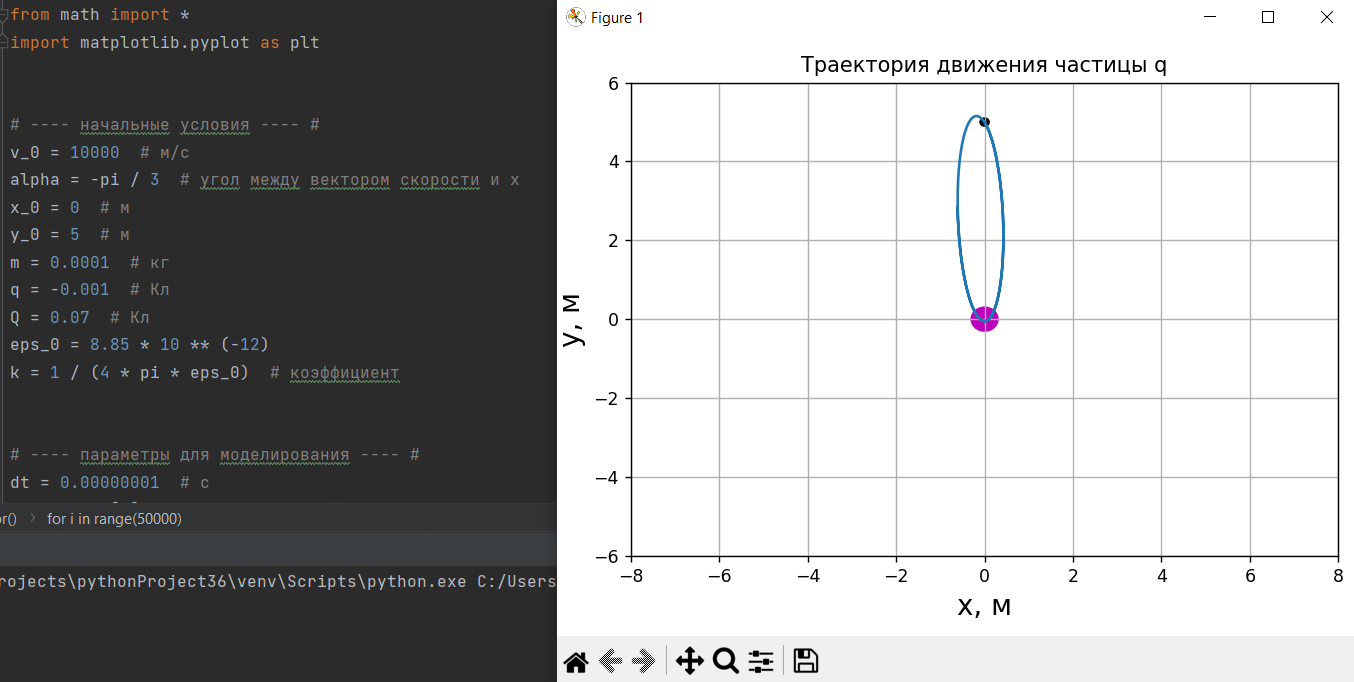
\includegraphics[width=0.92\linewidth]{gr/1.png}}
\caption{Траектрия 1 движения частицы $q$ при соответствующих параметрах.}
\end{figure}

\begin{figure}[h!]
\center{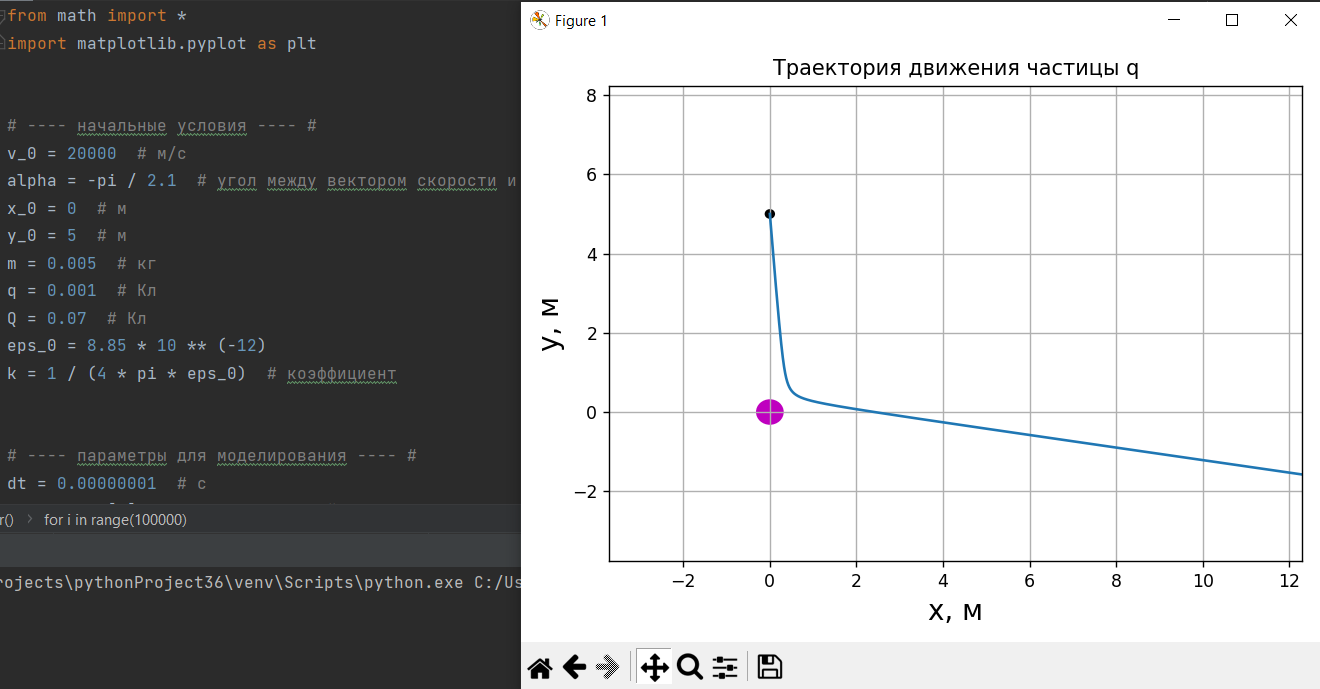
\includegraphics[width=0.92\linewidth]{gr/2.png}}
\caption{Траектрия 2 движения частицы $q$ при соответствующих параметрах.}
\end{figure}

\begin{figure}[h!]
\center{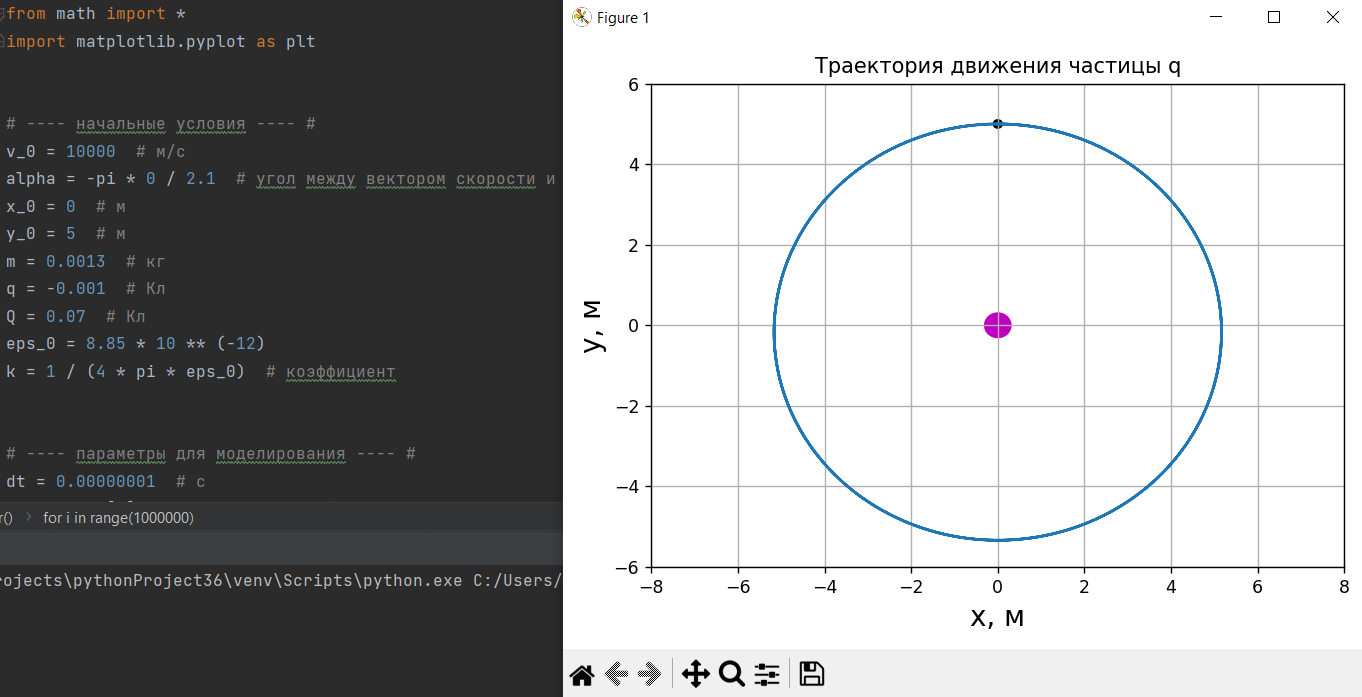
\includegraphics[width=0.92\linewidth]{gr/3.png}}
\caption{Траектрия 3 движения частицы $q$ при соответствующих параметрах.}
\end{figure}

\begin{figure}[h!]
\center{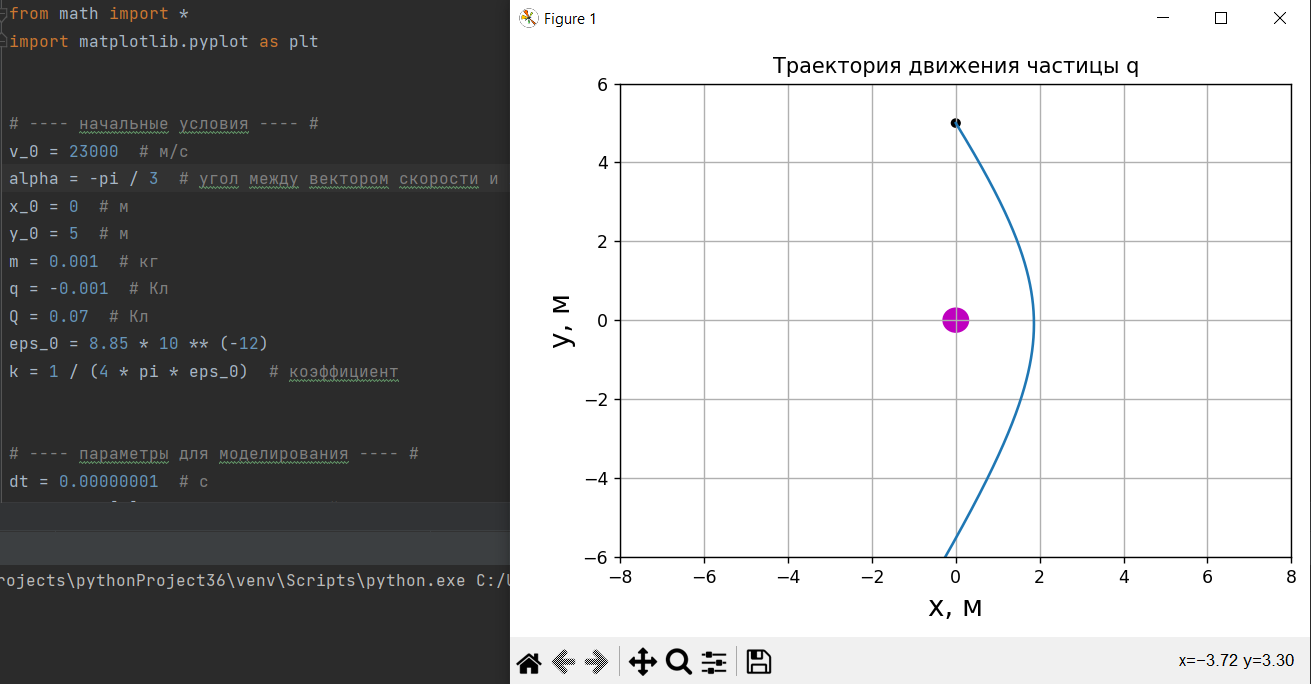
\includegraphics[width=0.92\linewidth]{gr/4.png}}
\caption{Траектрия 4 движения частицы $q$ при соответствующих параметрах.}
\end{figure}

\begin{figure}[h!]
\center{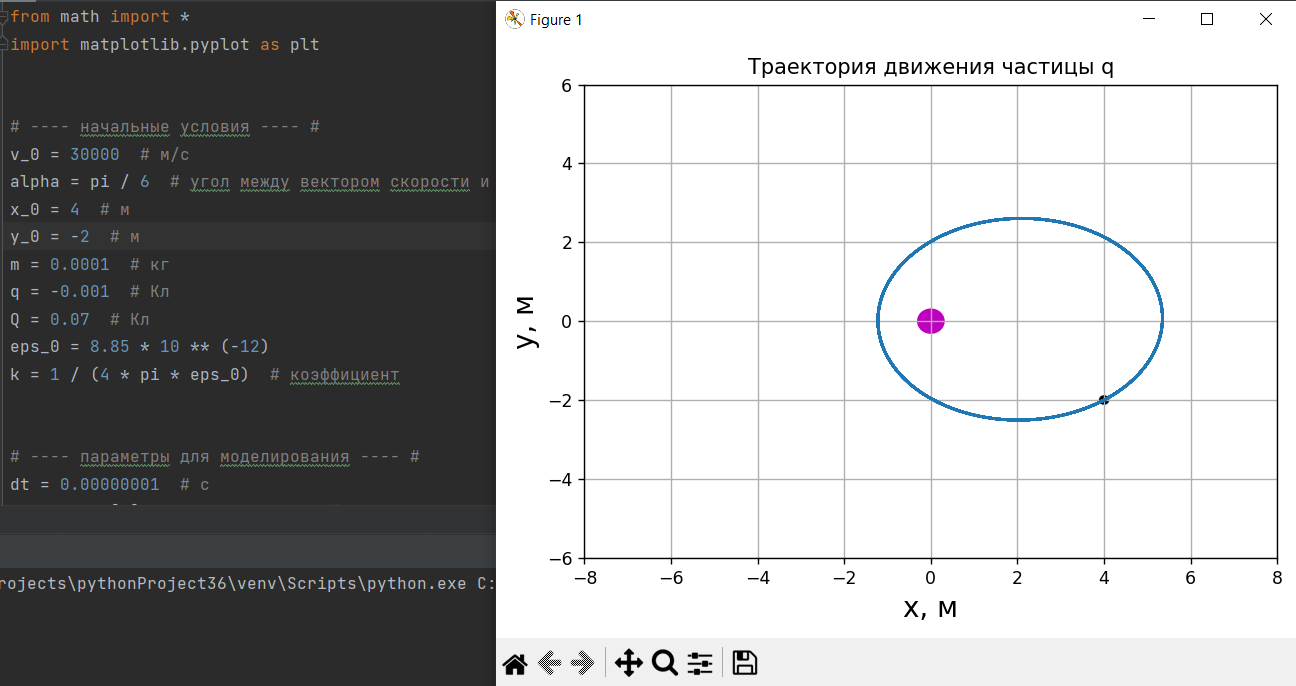
\includegraphics[width=0.92\linewidth]{gr/5.png}}
\caption{Траектрия 5 движения частицы $q$ при соответствующих параметрах.}
\end{figure}



\newpage

\newpage
\,
\newpage
Для визуализации был написан код на языке \textit{Python}. \\
Код расположен на \href{https://github.com/a-nechaeva/phys_project_2/blob/main/python_code/electric_move.py}{\textbf{GitHub}}.

\section{Анализ результатов работы и вывод.}
В процессе работы мы наглядно убедились что силы электрического взаимодействия очень велики. Они легко притягивают тело летящее с огромной скоростью.\\
Моделируя тела разных зарядов а точке наибольшего сближения мы столкнулись с очень большими значениями скорости и ускорения. Для правильного отображения траектории было необходимо использовать очень малое приращение времени.\\
Для разноимённых зарядов нам удалось наблюдать траекторию подвижного тела в виде эллипса, окружности и гиперболы. К сожалению увидеть параболу не получилось, необходимы точные значения.\\
Как итог, поведение заряженной частицы в электрическом поле другой вполне предсказуемо и легко рассчитывается для любых значений скоростей, зарядов, масс, стартовых точек и направлений начальной скорости.
\end{document}













